\section{Implementation and Evaluation}

The prototype implementation can be found on GitHub.
\begin{displayquote}
\url{https://github.com/kc1212/consensus-thesis-code}
\end{displayquote}
It implements the three protocols and the Extended TrustChain.
We also implement two optimisations---privacy preserving validation protocol using compact blocks (\Cref{sec:compact})
and optimised validation protocol using cached agreed fragments (\Cref{sec:caching}).
It is written in the event driven paradigm, using the Python programming language\footnote{\url{https://www.python.org/}}.
The cryptography primitives we use are SHA256 for hash functions and Ed25519 for digital signatures.
Both of which are provided by libnacl~\footnote{\url{https://pypi.python.org/pypi/libnacl}}.


\subsection{Experimental setup}
\label{sec:experimental-setup}

We run the experiment on the DAS-5\footnote{\url{https://www.cs.vu.nl/das5/}} with up to 1200 nodes.
Every node makes a transaction with a random node twice every second.
Since Bitcoin transactions are approximately 500 bytes~\cite{txsize},
we use a uniformly random transaction size sampled between 400 and 600 bytes.

To coordinate nodes on many different machines,
we employ a discovery server to inform every node the IP addresses and port numbers of every other node.
It is only run before the experiment and is not used during the experiment.

\subsection{Linear Global Throughput}

The global throughput results are shown in~\Cref{fig:global-throughput}.
Evidently, the throughput has a linear relationship with the population size.
This result is a strong indication of the horizontal scalability which we aimed to achieve.

\begin{figure}[h]
  \centering
  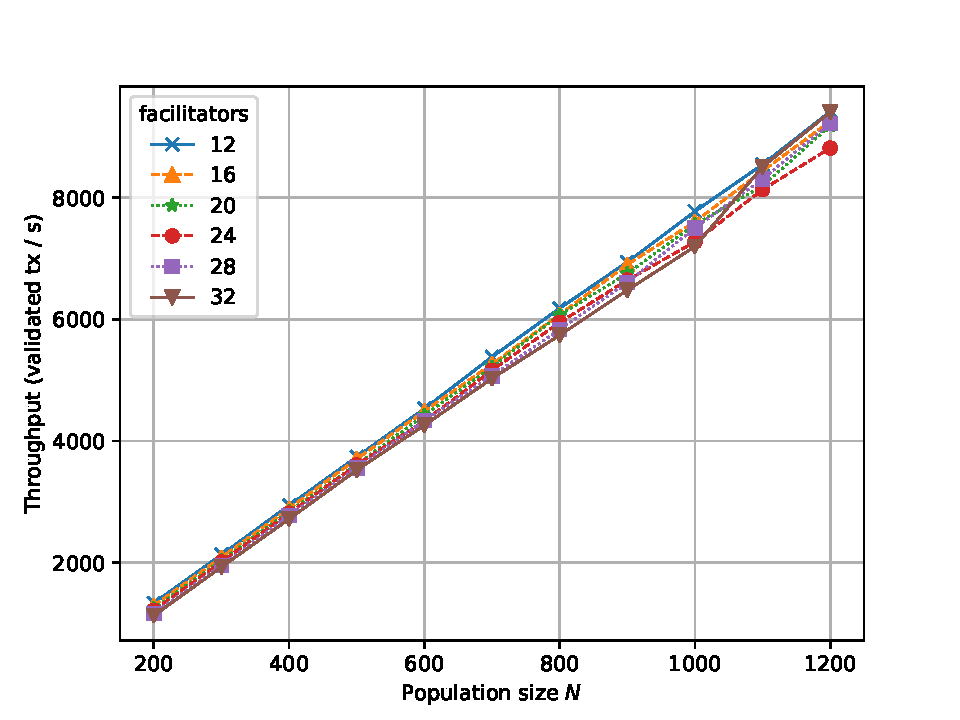
\includegraphics[width=\linewidth]{neighbour-random/throughput-vs-population}
  \caption{Global throughput increases as the population increases when every node transact at the same rate.
  Using fixed neighbours results in a higher throughput because of the caching mechanism.}
  \label{fig:global-throughput}
\end{figure}


